\documentclass[conference, a4paper]{IEEEtran}
\IEEEoverridecommandlockouts
%% The preceding line is only needed to identify funding in the first footnote. If that is unneeded, please comment it out.
\usepackage{cite}
\usepackage{amsmath,amssymb,amsfonts}
\usepackage{algorithmic}
\usepackage{graphicx}
\usepackage{textcomp}
\usepackage{xcolor}
\def\BibTeX{{\rm B\kern-.05em{\sc i\kern-.025em b}\kern-.08em
    T\kern-.1667em\lower.7ex\hbox{E}\kern-.125emX}}
\begin{document}

\title{Comparative analysis on Computing Disparity map \\
{\footnotesize \textsuperscript{*}Note: Sub-titles are not captured in Xplore and
should not be used}
%\thanks{Identify applicable funding agency here. If none, delete this.}
}

\author{\IEEEauthorblockN{1\textsuperscript{st} Chitra Suresh}
\IEEEauthorblockA{\textit{dept. name of organization (of Aff.)} \\
\textit{name of organization (of Aff.)}\\
City, Country \\
email address}
\and
\IEEEauthorblockN{2\textsuperscript{nd} Given Name Surname}
\IEEEauthorblockA{\textit{dept. name of organization (of Aff.)} \\
\textit{name of organization (of Aff.)}\\
City, Country \\
email address}
%\and
%\IEEEauthorblockN{3\textsuperscript{rd} Given Name Surname}
%\IEEEauthorblockA{\textit{dept. name of organization (of Aff.)} \\
%\textit{name of organization (of Aff.)}\\
%City, Country \\
%email address}
%\and
%\IEEEauthorblockN{4\textsuperscript{th} Given Name Surname}
%\IEEEauthorblockA{\textit{dept. name of organization (of Aff.)} \\
%\textit{name of organization (of Aff.)}\\
%City, Country \\
%email address}
%\and
%\IEEEauthorblockN{5\textsuperscript{th} Given Name Surname}
%\IEEEauthorblockA{\textit{dept. name of organization (of Aff.)} \\
%\textit{name of organization (of Aff.)}\\
%City, Country \\
%email address}
%\and
%\IEEEauthorblockN{6\textsuperscript{th} Given Name Surname}
%\IEEEauthorblockA{\textit{dept. name of organization (of Aff.)} \\
%\textit{name of organization (of Aff.)}\\
%City, Country \\
%email address}

}

\maketitle

\begin{abstract}
Stereoscopic images or stereo pair image consists of two images of the same object/ terrain taken slightly horizontally separated points, known as left view and the right view. Generally an image contains multiple objects and the objects situated at different depth show different displacement in these two images. The disparity for stereoscopic images is the horizontal distance between two matching pixel and the disparity-map is an image showing disparity of each pixel. . This map is indicative of the stereo information. In this paper we computed disparity map using Minimum Index method and the results are compared with the 'build in function of Matlab,  method and Minimum sum Belief propagation method. The computation disparity map at different disparity level is explored. The computational error estimation and runtime analysis is also performed at disparity level sixteen.


\end{abstract}

\begin{IEEEkeywords}
Stereo Image, Disparity, Disparity Map
\end{IEEEkeywords}

\section{Introduction}
The stereoscopic images or stereo pair image consists of two images of the same scene taken slightly horizontally separated points from the left view and the right view. The horizontal displacement of an object left and right view depends on the distance from the object to the camera view points. The disparity for stereoscopic image is horizontal distance between two matching pixel. The disparity map is horizontal pixel distance for each pixel coordinates. The Depth map or Disparity map is a gray scale image which is highly compressed. The Depth map or Disparity map shows distance rather than texture. If shift of pixel between  right and left stereo image is more than object looks darker which is located far away from camera and if shift is less than object is bright i.e. object close to the camera.\\
There are various methods to find Disparity map or Depth map which are Area-based, Feature- based and Global based methods. The Area and Feature based methods are based on intensity profile. The  constrain in Area- based method is to find the optimal size of the window. The Feature-based method is  restricted to feature which  yields sparse disparity map. The Global method is  based on Bayesian approach to finds disparity as an energy minimization problem.\\
Accurate disparity information is very significant as it can be used to reconstruct 3D model sequences which can be used either for information transfer or for entertainment.
It also finds application in robotic navigation\\
In Robotic application disparity map is used to navigate and to recognize object to separate occluded region in image components\\
Scientific application of Disparity Map is to extracts information from aerial surveys and for calculation of contour map.\\
In this paper we computed disparity map using three different methods which are Minimum Index Method ,  'Disparity Map' build in function from  computer vision tool box of Matlab and  Minimum Sum Belief propagation method. The error estimation shows that disparity map using Minimum Index method at disparity level sixteen is better than other two methods. The subjective analysis with respect to ground truth images shows that disparity map at disparity level sixty four is using Minimum Sum Belief propagation is more compensable to other two methods.
The run time for all three methods at sixteen disparity level are computed .The run time for minimum index  method is twice that of build in function  method of matlab.\\
 This paper is organized as follows: Literature survey is given in section II, overview of method used is explained in section III, experimental results shown in section IV and its discussion elaborated in section V and conclusion is given in section VI



\section{	LITERATURE SURVEY }
The method used in [1] "Adaptive support -weight approach for correspondence search" is area based local method to generate depth map or disparity map. The proposed method is based on Gestalt grouping in which support weight is based on similarity and proximity and is proportional to the strength of the grouping. The group of similarity is calculated by means of Euclidean distance whereas group of proximity is by means of Laplacian Kernel.\\
The method used [7] in "A Region Based Stereo Matching Algorithm Using Cooperative Optimization "is region based window based stereo matching algorithm using cooperative optimization. In cooperative optimization regions are selected using color statistics and constrains on smoothness and occlusion between adjacent regions.
The homogeneous color segmentation and window based plane fitting techniques are used in Cooperative Optimization.\\
The method used in [2] "A New Approach for Disparity Map Estimation from stereo Image Sequences using Hybrid Segmentation Algorithm" is feature based local method to generate depth map or disparity map. The estimation of Disparity map is by using K-mean square algorithm and hybrid segmentation algorithm. The criteria used for K-mean is by minimizing the distance between data and cluster centroid. The segmentation algorithm extracts feature by Scale Invariant Feature Transform (SIFT) and Sum of Absolute Difference (SAD).\\
The method used in [3] "A Comparative Study of Energy Minimization Methods for Markov Random Fields" is global based method to generate depth map or disparity map. The method used is energy minimization problem on rectangular grid of pixels where energy expressed as data term and smoothness term.\\
The method used in "Efficient Loopy Belief Propagation using the Four Color Theorem"[12] is global stereo matching method to compute disparity map or depth map.
The Four-Color Theorem based on the max-product belief propagation technique used to solve Markov Random Field formulation to minimize energy.\\
The method used in research paper  "Comparison of graph cuts with BP for stereo using identical MRF parameters"[6] is global method. The disparity image  computed by modeling Markov Random Field and by using optimization algorithm such as Graph cut and Belief Propagation. These two algorithms allow fast and approximate solution to MRF which are powerful tools for modeling vision problems. So one system can improvement over the other is particularly to its choice of an inference algorithm.



\section{OVER VIEW OF METHOD USED}
\textbf{The first method used} to compute disparity map is using MATLAB in build function "Disparitymap" in computer vision tool box. The algorithm used in matlab in build function is Semi Global Block matching algorithm [4] .The sum of absolute difference is applied for each block of pixel to enforces same disparity to neighboring blocks.\
The steps used in MATLAB in build function method are\begin{enumerate}
                                                       \item 	{Reading left and right test stereo images}
                                                       \item {Keeping block size 15 and default method used Semi Global}
                                                       \item {Finding disparity map using "DisparityMap" function}
                                                       \item {Disparity range kept is 16}
                                                       \item {Display disparity map}

                                                     \end{enumerate}

\textbf{The second method used }to compute disparity map is minimum index method. In Minimum indexed   method, Minimum sum of absolute difference function is used. The intensity value or pixel value is shifted by disparity range or level either in left stereo image or to right stereo image. \\In proposed indexed method right stereo image is shifted by disparity range or level. When  minimum occurs in shifted values which is considered as disparity. The stereo pair or stereo images are rectified images so that horizontal scanning is performed on these images. The mathematical description of proposed method is given below.\\
The general function used as cost function for stereo pair image   to find disparity map is:
\begin{equation}
Cost function  (C _{f}) = |I_{L} -I_{R} |                                                                \label{eq}
\end{equation}
Where
\begin{itemize}
  \item { $I_{L}$ is left stereo image} 
  \item {$I_{R}$ is right stereo image}
\end{itemize}
In Minimum Index method Minimum sum of Absolute Difference (SAD) is used.
\begin{equation}
Cost function  (C _{f1}) = |I_{L} -I_{R-d} |         \label{eq}
\end{equation}
Where d is disparity range or level:\\
The disparity value is decided when, minimum difference in pixel values is observed
\begin{equation}
 f(z) = min(C _{f1})    \longrightarrow   1<z<d  \label{eq}
\end{equation}
                                          

where
\begin{itemize}
  \item { z is minimum disparity value}
  \item {z varies $1>z<d$ }
\end{itemize}
The algorithmic steps in Minimum Index method

\begin{itemize}
  \item { Reading left and right test stereo images   }
  \item {	Shifting right matrix with each disparity value.}
  \item {	Perform absolute difference between left and right matrix }
  \item {	Finding minimum difference in pixel values}
  \item {	Display disparity map }
\end{itemize}

\begin{table}[htbp]
\caption{Table Type Styles}
\begin{center}
\begin{tabular}{|c|c|c|c|}
\hline
\textbf{Table}&\multicolumn{3}{|c|}{\textbf{Table Column Head}} \\
\cline{2-4}
\textbf{Head} & \textbf{\textit{Table column subhead}}& \textbf{\textit{Subhead}}& \textbf{\textit{Subhead}} \\
\hline
copy& More table copy$^{\mathrm{a}}$& &  \\
\hline
\multicolumn{4}{l}{$^{\mathrm{a}}$Sample of a Table footnote.}
\end{tabular}
\label{tab1}
\end{center}
\end{table}
\section{EXPERIMENTAL RESULTS}
The test stereo images used for experimental analysis are from Middlebury computer vision web site (vision.middlebury.edu). The ground truth image for each test stereo image is used for comparing performance of disparity map. [13].The software used for programming is MATLAB version 15.\
The disparity map is computed using minimum index method, MATLAB in build function "DisparityMap" and using Minimum sum Belief Propagation method for disparity level 16.The different disparity map for various test stereo images for all 3 methods with input stereo image and ground truth are shown in figure3

\begin{figure}[htbp]
\centering
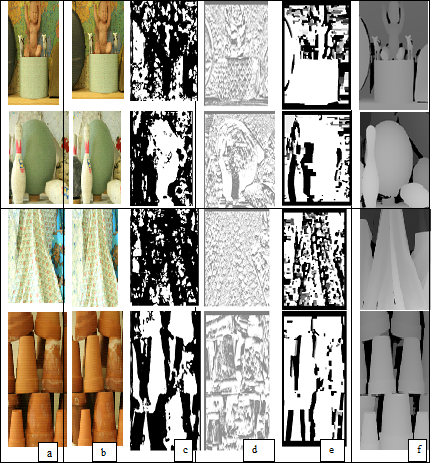
\includegraphics[width=3in]{3METHODS.eps}
\caption{(a)Left Image  (b) Right Image (c) In build MATLAB function method(d) Minimum Index Method(e) Minimum Sum Method         (f) Ground   truth     }
\label{fig_sim}
\end{figure}

The computational estimation mean square error (MSE) is calculated with respect to ground truth for all computed disparity map. The estimated MSE per total number of pixel are shown in table1

\begin{figure}[htbp]
\centering
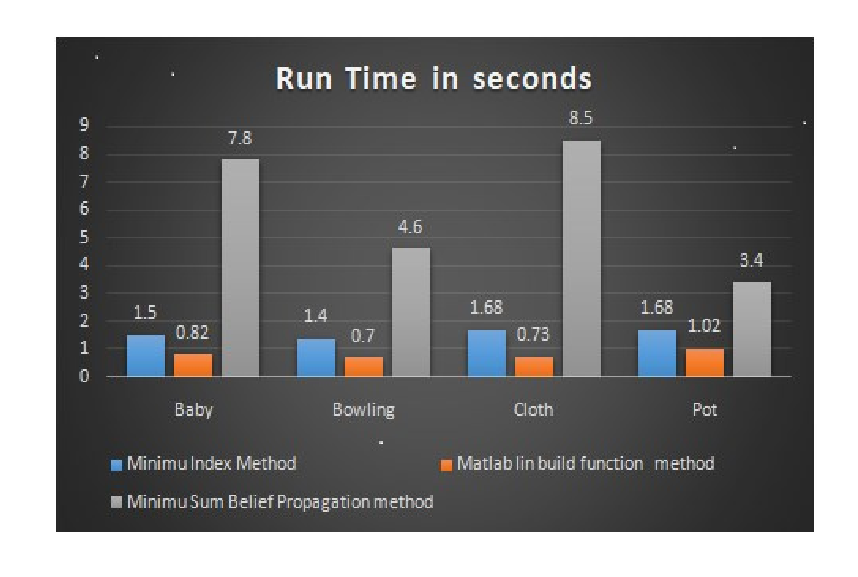
\includegraphics[width=3in]{bargraph.eps}
\caption{(a)Left Image  (b) Right Image (c) In build MATLAB function method(d) Minimum Index Method(e) Minimum Sum Method         (f) Ground   truth     }
\label{fig_sim}
\end{figure}







\begin{figure}[htbp]
\centering
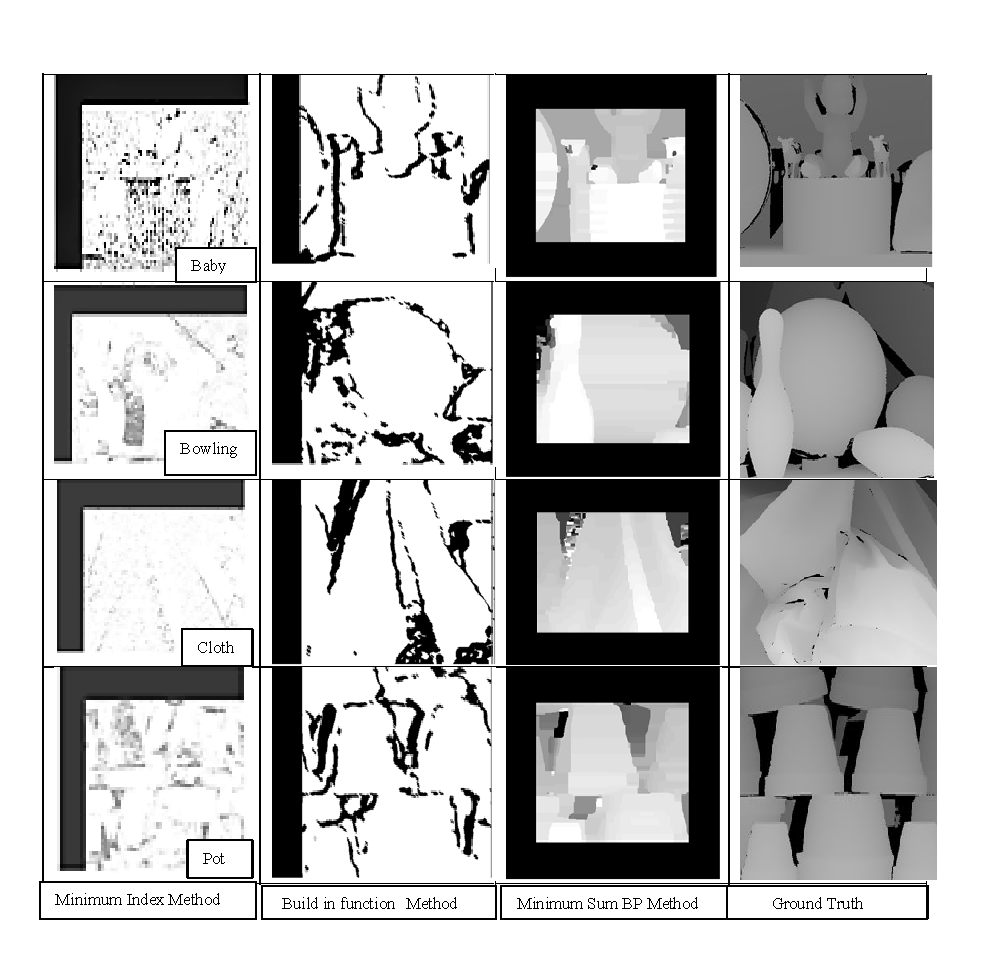
\includegraphics[width=3in]{diagram2.eps}
\caption{(a)Left Image  (b) Right Image (c) In build MATLAB function method(d) Minimum Index Method(e) Minimum Sum Method         (f) Ground   truth     }
\label{fig_sim}
\end{figure}





%\begin{figure}
%  % Requires \usepackage{graphicx}
%  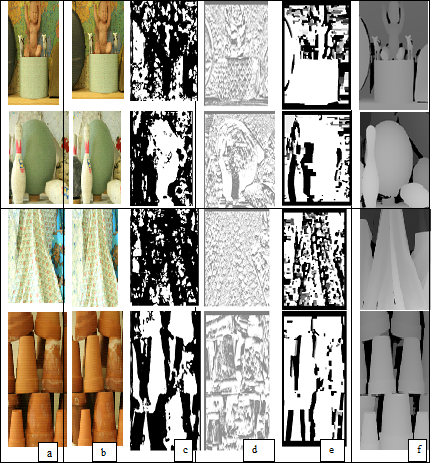
\includegraphics{3METHODS.png}
%  \caption{}\label{}
%\end{figure}



%\begin{figure}[htbp]
%\centerline
%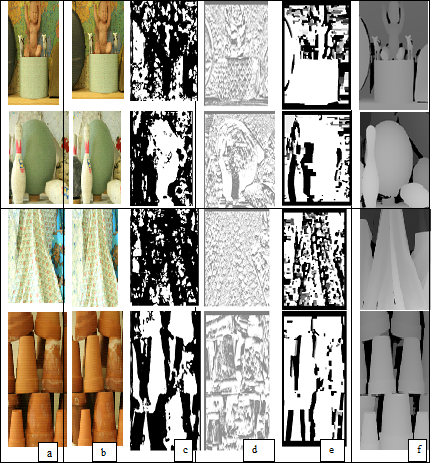
\includegraphics{3METHODS.png}
%\caption{Example of a figure caption.}
%\label{fig}
%\end{figure}




%\begin{figure}[htbp]
%\centerline{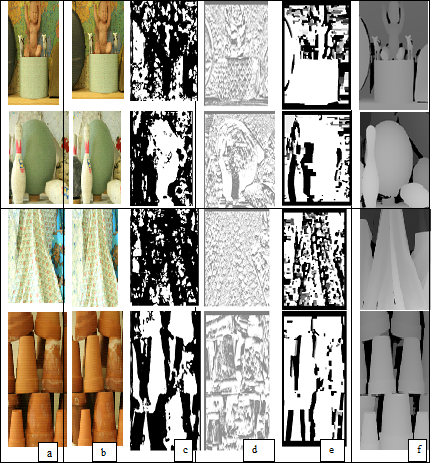
\includegraphics{3METHODS.png}}
%\caption{Example of a figure caption.}
%\label{fig}
%\end{figure}




\section{DISCUSSION}
In first analysis, disparity map is computed at disparity level16 using Minimum Index,"DisparityMap" MATLAB in build function and Minimum Sum Belief Propagation methods. The computational error estimation i.e. Mean Square Error per total number of pixels is less for all test stereo image using Minimum Index than,"DisparityMap" function and Minimum Sum Belief Propagation.
The run time analysis shows that for all test stereo images at disparity level sixteen  using matlab inbuilt function method takes less time where as the run time using minimum index method takes twice as compare to MATLAB in build function method. The time taken to run minimum sum belief propagation is more compare to other two methods.\\
In second analysis disparity level is increased to sixty four for all methods. The performance analysis is subjectively by human perception with respect to ground reality image, which shows that disparity map computed using  Minimum Sum Belief Propagation is better than Minimum Index than ,"DisparityMap" function. When disparity level is increased to sixty four MATLAB in build function detects the edges of the objects in disparity map. The constrain in minimum Index is that when disparity level is increased to sixty four is that to find minimum index value in disparity map


\section{Conclusion}
The disparity map is computed using Minimum Index method, MATLAB in build function from computer vision tool box and Minimum Sum Belief Propagation method at different disparity levels. The computational error estimation and subjective analysis by human perception shows that minimum index method is better at disparity level   sixteen  than other two methods.\\
The   second subjective analysis by human perception with respect to ground truth shows that sharpness of disparity map computed by Minimum Sum Belief Propagation method at disparity level sixty four is better than other two methods.\\
The further   study can be done to improve performance in minimum index method using smoothing filters. In detail study of minimum sum belief propagation is required as future study

\section*{Acknowledgment}

The preferred spelling of the word ``acknowledgment'' in America is without
an ``e'' after the ``g''. Avoid the stilted expression ``one of us (R. B.
G.) thanks $\ldots$''. Instead, try ``R. B. G. thanks$\ldots$''. Put sponsor
acknowledgments in the unnumbered footnote on the first page.

%\section*{References}



\begin{thebibliography}{00}
\bibitem{b1} 	L. kuk-Jin Yoon, In Sokweon, "Adaptive support -weight approach for correspondence search,"  IEEE Trans- actions on pattern analysis and machine Intelligence Vol. 28,no.4,April 2006,pp 650-651.
\bibitem{b2} 	Patrik Kamencay,Martina Zachariasova,Martin Brezman,Roman Jarina,Robert Hudec,Miroslav Benco,Slavomir Matuska, "A New Approach for Disparity Map Estimation from stereo Image Sequences using Hybrid Segmentation Algorithm", International Journal of Modern Engineering Research,Vol.2,Issue 5,Sep-Oct 2012 ,pp3201-3206
\bibitem{b3} 	R.  Szeliski,  R.  Zabih,  D.  Scharstein,  O.  Veksler,  V.  Kolmogorov,  A.  Agarwala,  M.F. Tappen and C. Rother,  "A Comparative Study of Energy Minimization  Methods for Markov Random Fields", IEEE Trans. Pattern Anal. Mach. Intell., vol. 6, no. 30, (2008), pp. 1068-1080.
\bibitem{b4}	Http://in.mathworks.com/help/vision/ref/disparity.html
\bibitem{b5} 	Brad Hiebert-Treuer,SarriAl Nashashibi and Daniel Scharstein,Middlebury stereo vision pages, http://Vision.middlebury.edu
\bibitem{b6} 	Tappen,M.F.andFreeman,W.T.,"Comparision of graphcuts with BP for stereo using identical MRF parameters",In IEEE International conference on computer vision
\bibitem{b7} 	Zeng-Fu Wang and Zhi-Gang Zheng, "A region based stereo matching algorithm using cooperative optimization," 2008 IEEE Conference on Computer Vision and Pattern Recognition, Anchorage, AK,2008,pp.1-8.doi: 10.1109/CVPR.2008.4587456
\bibitem{b8}  	M. Z. Brown, D. Burschka, and G. D. Hager, "Advances in computational stereo," IEEE Transactions on Pattern Analysis and Machine Intelligence, vol. 25, no. 8, pp. 993-1008, 2003
\bibitem{b9} 	KomalD.Bhavsar, Virendra Singh," Analysis of Disparity Map for stereo Matching Algorithm", International Journal for scientific Research  and Development,Vol.1,IIsue 11,2014,ISSN(online):2320613
\bibitem{b10} W. D. Hu, K. Zhang, L. F. Sun, J. Y. Li, Y. J. Li and S. Q. Yang, "Virtual Support Window for Adaptive-weight Stereo Matching", IEEE Visual Communications and Image Processing (VCIP), (2011) November 6-9, pp. 1-4, Tainan, Taiwan.
\bibitem{b11} 	Dan  Yuan,  "Understanding  Belief  Propagation  And  Its  Applicatons ",  Department Of Computer Engineering ,University Of California.
\bibitem{b12}	Timofte R., Van Gool L. (2013) Efficient Loopy Belief Propagation Using the Four Color Theorem. In: Farinella G., Battiato S., Cipolla R. (eds) Advanced Topics in Computer Vision. Advances in Computer Vision and Pattern Recognition. Springer, London https://doi.org/10.1007/978-1-4471-5520-1-11
\bibitem{b13} Colin Doutre and PanosNasiopoulos," A Stereo matching Datacost Robust to Blurring",IEEE 17th International conference on Image Processing, September 26-29, 2010,Hong Kong
\bibitem{b14}	R. Klette and S. Morales, "Prediction Error Evaluation of Various Stereo Matching Algorithms on Long Stereo Sequences," 2009.
\bibitem{b15} 	https://github.com/daviddoria/Tutorials/blob/master/BeliefPropagation/- BeliefPropagation.pdf?raw=true
\bibitem{b16}	https://vision.middlebury.edu/stereo/data
\bibitem{b17}	LiCheng,TerryCaellu ,"Bayesian Stereo matching" ,Computer vision and Image understanding   http://www.elsevier.com/locate/eviu
\bibitem{b18}	Y. Boykov, O. Veksler and R. Zabih,"Markov Random Fields with Efficient Approximations, Proc. IEEE Int. Conf. Pattern Analysis and Machine Intelligence, (1998) June 23-25, pp. 648-655, Santa Barbara, CA, USA.
\bibitem{b19}	SomonHermann,ReinhardKlette" The Naked Truth about cost functions for stereo matching",http://www.mi.auckland.ac.nz/EISATS

\bibitem{b20}	G.Gerig,www.Sci.Utah.edu/gerig/CS6320-S2013/�../CS6320-cv-F2012-Rectification.pdf

\end{thebibliography}
\vspace{12pt}
%\color{red}
%IEEE conference templates contain guidance text for composing and formatting conference papers. Please ensure that all template text is removed from your conference paper prior to submission to the conference. Failure to remove the template text from your paper may result in your paper not being published.

\end{document}
